\chapter{基于PR目标的均衡优化}

本章聚焦于进一步提升多通道自适应均衡系统的性能与鲁棒性。在前述章节中，数字均衡器与多通道自适应均衡器的设计有效抑制了高密度AD光盘信道中的多维干扰。然而，均衡的性能仍然受到一个关键因素的制约——部分响应（PR）目标的选取。传统方法中，PR目标通常是依据经验或特定信道条件预先设定的固定值（如经典整数PR多项式），难以适应盘片差异、环境变化及长期老化等因素引起的信道特性漂移。为解决此问题，本章提出一种基于人工蜂群算法的最优PR目标搜索策略，旨在根据实际信号特征动态适配PR目标，从而突破固定PR目标的性能瓶颈，实现整体检测性能的进一步优化。

\section{现有PR目标及其局限性分析}

\begin{figure}[h]
	\centering
	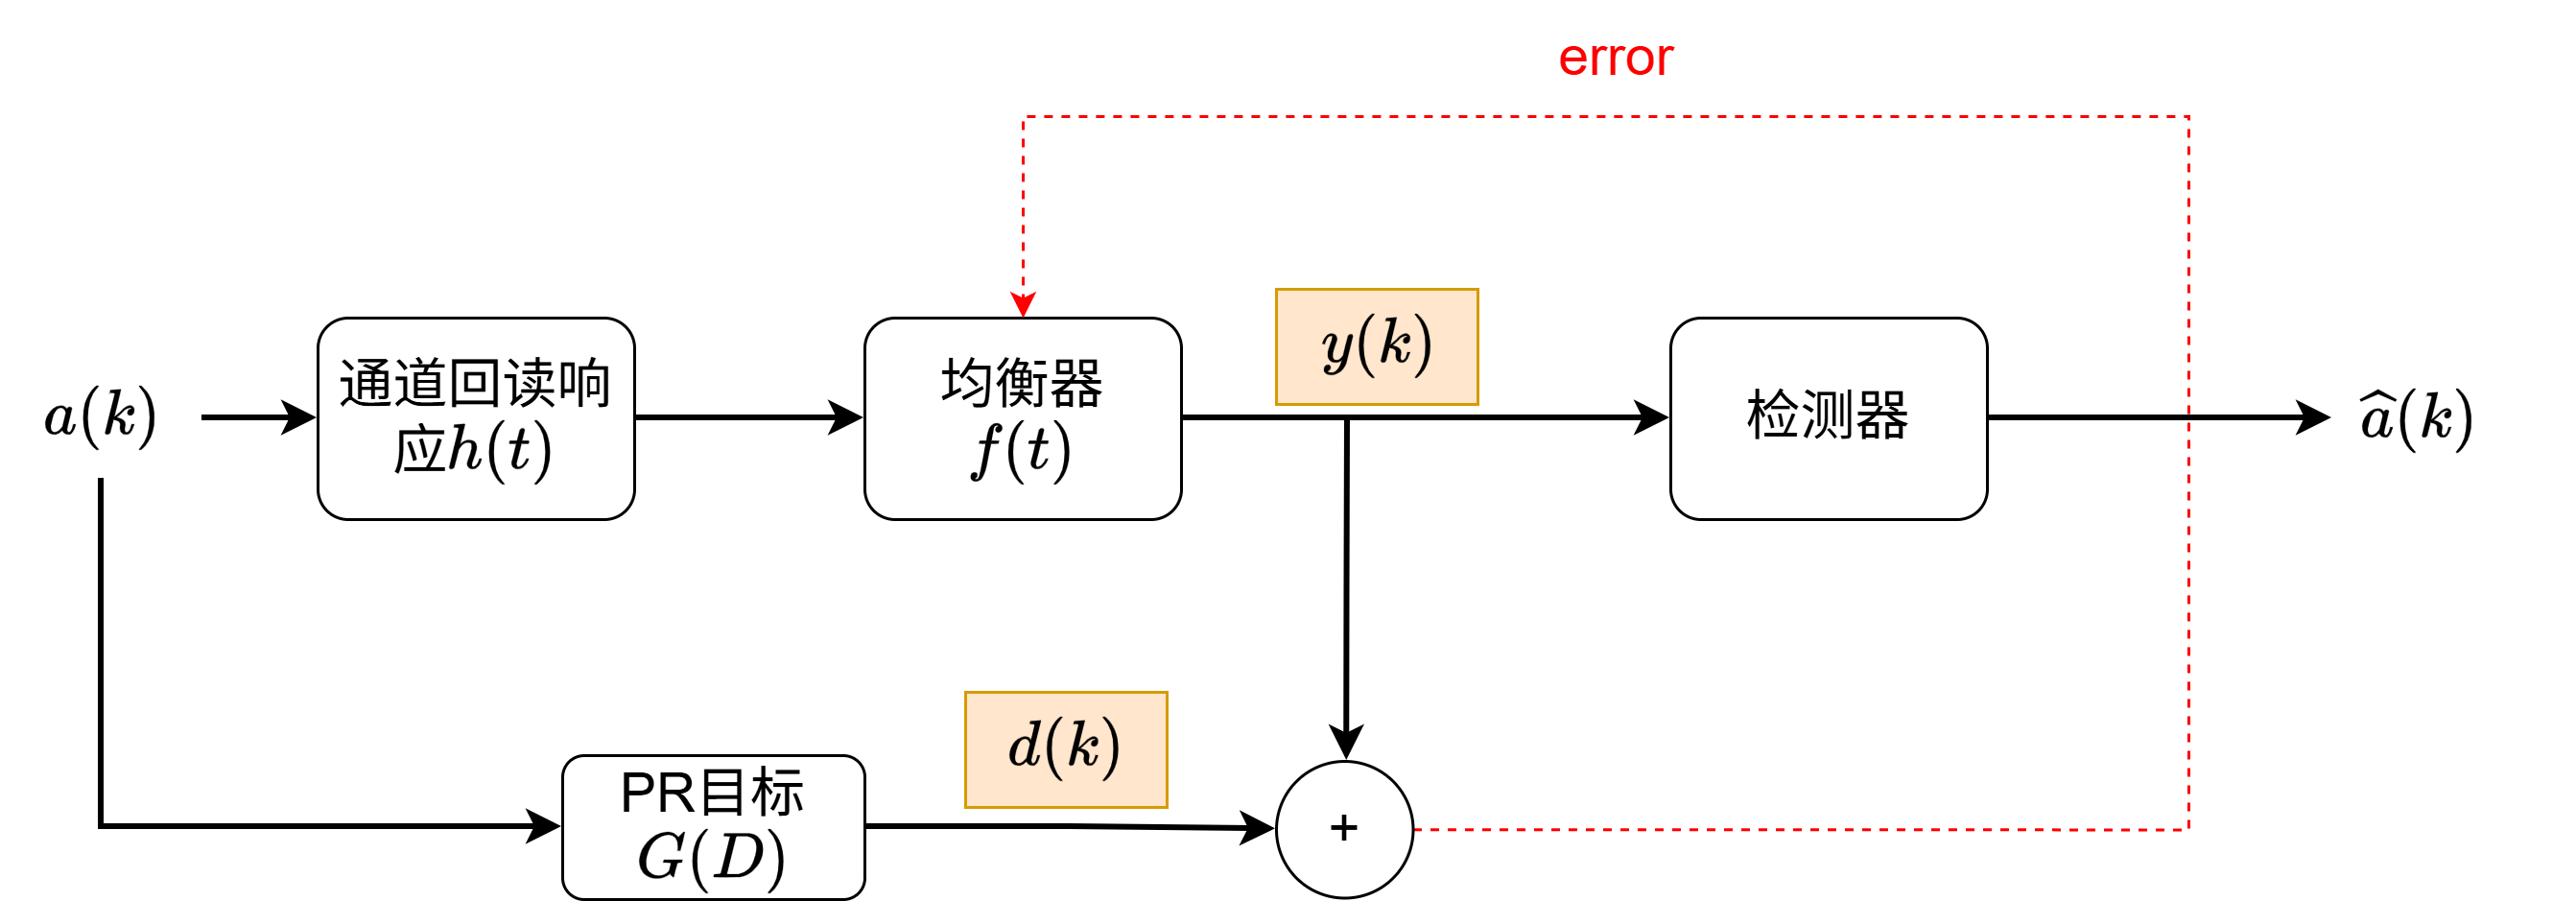
\includegraphics[width=\textwidth]{float/ch.cnn3/prml_framework.png}
	\caption{PRML系统框架图}
	\label{fig:prml_framework}
\end{figure}

PR目标在PRML检测框架中居于核心地位，其本质是对信道特性的一种受控描述，也是连接均衡器与检测器的关键纽带。PRML技术的基本原理可概括为两个紧密耦合的环节：信道塑造与序列检测。如图\ref{fig:prml_framework}所示的PRML系统框架图中，均衡器承担着将实际信道响应塑造成预设PR目标的任务。设实际光存储信道的冲激响应为$h(t)$，其频率特性受光学衍射极限、盘片结构等因素制约，通常表现为复杂的低通特性且难以直接用于检测。均衡器通过自适应滤波，使整体响应$h(t) * f(t)$逼近一个精心设计的、具有有限长度冲激响应的PR目标多项式$G(D)$。这一过程的核心意义在于：将原本复杂的、无限长的信道响应，转化为一种可控的、可预测的部分响应模式，从而为后续的最大似然序列检测创造有利条件。维特比检测器则基于此PR目标构建网格图，在受控的符号间干扰结构中搜索最大似然路径，最终恢复原始数据序列。

\begin{figure}[b]
	\centering
	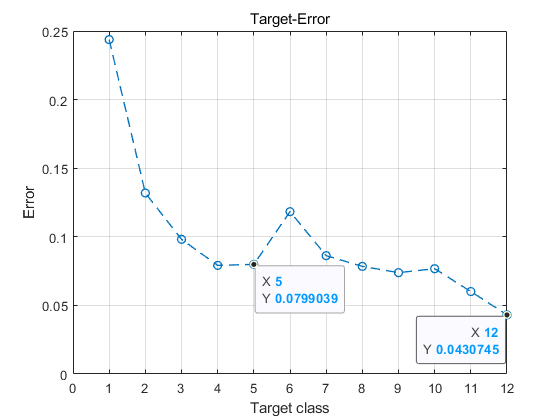
\includegraphics[width=0.65\textwidth]{float/ch.cnn3/pr_error_comparison.png}
	\caption{不同PR的均衡误差结果图}
	\label{fig:pr_error_comparison}
\end{figure}

PR目标的选择对系统性能产生着决定性影响，这种影响主要体现在两个相互关联的维度上。PR目标与实际信道特性的匹配程度直接决定了均衡后信号的残余干扰水平。当PR目标能够准确刻画信道的核心特征时，均衡后信号与理想目标信号之间的偏差较小，检测器获得更优的输入信号质量。反之，若PR目标与信道特性失配严重，均衡器为强行将信道响应塑造成不匹配的目标形态，导致均衡后信号信噪比恶化，残余干扰增加。图\ref{fig:pr_error_comparison}展示了采用表\ref{tab:pr_targets}里的PR目标进行均衡所获得的均衡误差结果。Target class编号为1的表示PR=[1,2,2,2,1]长度为5用在蓝光光盘中的PR目标。2~6为长度为7的PR目标；7~11为长度为9的PR目标，编号12为长度为11的PR目标。长度为11的PR均衡效果远优于较短长度PR均衡，但长度为5的PR中也有效果等同于甚至优于长度为7的PR。从图中可以清晰地观察到，PR目标的差异显著影响着最终的均衡的性能。其中，越长的PR目标能够取得明显优于其他目标的检测效果，但也有部分较短的PR取得了其他较长PR同样的效果，这直观地印证了PR目标与信道匹配程度对系统性能的关键作用。

\begin{table}[h]
	\centering
	\caption{整数 PR 目标表}
	\label{tab:pr_targets}
	\begin{tabular}{>{\centering\arraybackslash}p{0.8cm} l >{\ttfamily}l}
		\toprule
		\textbf{Index} & \textbf{Target name} & \textbf{Target array} \\
		\midrule
		1  & pr\_target5          & {[1,2,2,2,1]} \\
		\midrule
		2  & pr\_target7\_1       & {[1,5,6,8,6,5,1]} \\
		3  & pr\_target7\_2       & {[1,3,4,5,4,3,1]} \\
		4  & pr\_target7\_3       & {[2,4,6,7,6,4,2]} \\
		5  & pr\_target7\_4       & {[1,2,3,3,3,2,1]} \\
		6  & pr\_target7\_5       & {[1,1,2,2,2,1,1]} \\
		\midrule
		7  & pr\_target9\_1       & {[1,5,8,10,11,10,8,5,1]} \\
		8  & pr\_target9\_2       & {[2,7,9,14,16,14,9,7,2]} \\
		9  & pr\_target9\_3       & {[1,3,4,6,7,6,4,3,1]} \\
		10 & pr\_target9\_4       & {[2,6,8,11,14,11,8,6,2]} \\
		11 & pr\_target9\_5       & {[1,2,3,4,5,4,3,2,1]} \\
		\midrule
		12 & pr\_target11\_1      & {[3,6,9,13,16,17,16,13,9,6,3]} \\
		\bottomrule
	\end{tabular}
\end{table}

PR目标的长度与系数分布共同决定了检测器的实现复杂度与噪声容忍能力。从检测器设计的角度看，维特比算法的状态数目与PR目标的记忆长度呈指数关系——若PR目标长度为$L$，则网格图中的状态数为$2^{L-1}$。这意味着随着PR目标的增长，检测器的计算复杂度和存储需求将急剧增加。然而，PR目标长度的选择并非越短越好。较长的PR目标通常能够更精细地刻画信道特征，提供更高的噪声容忍度，但其带来的复杂度代价也必须纳入系统设计的权衡考量。理想的PR目标应当在有限的长度约束下，尽可能准确地匹配信道特性，实现性能与复杂度的最优平衡。


\subsection{ABC算法在PR目标搜索策略中的适配改进}

人工蜂群算法作为一种受自然界蜜蜂觅食行为启发的元启发式优化算法，因其结构简洁、控制参数少且全局搜索能力强，在解决复杂参数优化问题方面展现出显著优势。该算法由Karaboga于2005年首次提出\textcolor{red}{参考文献}，其核心思想源于对蜂群在觅食过程中所表现出的智能协作行为的观察与抽象，将优化问题的求解转化为人工蜂群在解空间中搜索最优食物源的过程，从而实现对复杂目标函数的高效优化。将其应用于光盘信号处理领域中的PR目标搜索问题，需要针对问题的物理特性和约束条件进行精心的适配改进，以确保算法能够高效、稳定地搜索到符合实际意义的优化解。

人工蜂群算法的基本框架模拟了蜂群中三类角色——雇佣蜂、观察蜂与侦察蜂——的协同工作模式。雇佣蜂对应着当前已经发现的解（食物源），其主要职责是在已知解附近进行精细化的邻域搜索，以期发现更优的解。每个雇佣蜂与一个特定的食物源相关联，并在该食物源的邻域内执行局部搜索操作，若发现的新解优于当前解，则完成解的替换。同时，雇佣蜂在完成搜索后，会通过一种抽象化的“摇摆舞”机制，将食物源的质量信息传递给观察蜂，这种信息传递为后续的选择过程提供了依据。观察蜂则扮演着开发者的角色，它们依据雇佣蜂传递的信息，以轮盘赌选择的方式从现有解集中挑选出优质食物源进行重点开发。这种选择机制使得质量更优的解获得更高的被选择概率，从而引导更多的搜索资源集中于有潜力的解区域，实现局部开发的深度强化。观察蜂在选定食物源后，同样会在其邻域内执行局部搜索操作，并通过贪心策略决定是否更新解。侦察蜂则承担着全局探索的职责，它们负责监控所有食物源的更新状态，当某个食物源在连续预设次数的迭代中均未得到改进时，判定该区域已陷入局部最优，此时侦察蜂将随机生成一个新的食物源替代原有解，从而为算法注入新的搜索活力，避免因过度集中于局部区域而导致搜索停滞。这一机制通过引入随机扰动，确保了算法在全局空间中的持续探索能力，有效平衡了局部开发与全局探索之间的矛盾。

上述三类角色的分工协作构成了人工蜂群算法的完整搜索框架。算法\ref{alg:abc_framework}以伪代码形式展示了ABC算法的核心逻辑结构，清晰地呈现了雇佣蜂、观察蜂与侦察蜂三类角色的协同工作流程。

\begin{algorithm}[H]
	\caption{人工蜂群算法基本框架}
	\label{alg:abc_framework}
	\begin{algorithmic}[1]
		\STATE 初始化种群规模$N_p$、维度$T$、最大迭代次数$I_{\max}$、限制次数$L$
		\STATE 随机初始化$N_p$个候选解$\{x_i\}_{i=1}^{N_p}$，计算其适应度
		\WHILE{迭代次数 $< I_{\max}$}
		\STATE \textbf{雇佣蜂阶段}
		\FOR{每个雇佣蜂$i$}
		\STATE 在$x_i$的邻域内生成新解$v_i$
		\STATE 计算$v_i$的适应度，若优于$x_i$则替换
		\ENDFOR
		\STATE 计算每个解被选择的概率$p_i$
		\STATE \textbf{观察蜂阶段}
		\FOR{每个观察蜂}
		\STATE 依据概率$p_i$选择解$x_i$
		\STATE 在$x_i$的邻域内生成新解$v_i$
		\STATE 计算$v_i$的适应度，若优于$x_i$则替换
		\ENDFOR
		\STATE \textbf{侦察蜂阶段}
		\FOR{每个解$x_i$}
		\IF{$x_i$连续$L$次未更新}
		\STATE 随机生成新解替换$x_i$
		\ENDIF
		\ENDFOR
		\STATE 记录当前最优解
		\ENDWHILE
		\RETURN 全局最优解
	\end{algorithmic}
\end{algorithm}

将上述算法框架应用于PR目标搜索问题，需要针对问题的特殊性进行系统性的定制化设计。这些改进贯穿算法的各个阶段，共同确保搜索过程的效率与解的有效性。

在解的编码与初始化阶段，每个候选PR目标被编码为一个长度为$T$的实数向量，其中维度$T$被设定为奇数。这一设定源于PR目标的物理意义——向量中的每个系数对应于光学头对不同位置记录符的响应强度，响应中心位置应为强度最大值点，响应强度向两侧依次递减。这种编码方式使解向量与实际的物理响应特性形成直观对应。初始化过程兼容两种方式：一方面，采用随机生成的方式产生初始种群，以保障解的多样性，使算法具备探索未知解空间的能力；另一方面，允许人为指定经典PR目标（如$[1,2,2,2,1]$、$[1,3,4,4,3,1]$等）作为初始个体，这种设计使算法能够在继承已有领域知识的基础上进行优化，既避免了完全随机搜索的盲目性，又为突破传统固定目标的性能局限提供了可能。

针对解空间的结构特性，算法引入了专门的约束机制以确保搜索到的解符合实际物理意义。该约束机制在个体的每次更新过程中发挥作用，保证每个PR目标序列的系数呈“递增再递减”的单峰分布形态，即从序列两端向中心位置系数值单调递增，且在中心位置达到最大值后向另一端单调递减，这与光学头响应强度的实际分布规律相一致；将所有系数值限制在$[0,1]$区间内，实现归一化处理，这既避免了系数幅值过大导致的数值不稳定问题，也使不同长度、不同量级的PR目标具备可比性。通过在雇佣蜂和观察蜂的邻域搜索后施加上述约束，算法能够确保每次变异产生的候选解在结构上具有合理性，从而有效缩小搜索空间、提升收敛效率。

目标函数的设计是算法适配改进的关键环节。本文采用Kullback-Leibler散度作为衡量PR目标优劣的量化指标。KL散度从信息论角度度量两个概率分布之间的差异程度，将其应用于PR目标评价的基本思路是：对于某一候选PR目标，将其与写入信号卷积生成理想信号$D_k$，同时获取当前均衡后的回读信号$Y_k$，通过计算$Y_k$与$D_k$的概率分布之间的KL散度，来评估该PR目标下信号分布的匹配程度。KL散度越小，表明均衡后信号与理想信号的分布越接近，即该PR目标与当前信道特性的适配度越高。其计算公式为：
\begin{equation}
	\text{distance} = D(D_k \parallel Y_k) = \sum_{i \in X} D_k(i) \cdot \log \left( \frac{D_k(i)}{Y_k(i)} \right)
\end{equation}

在实际计算过程中，KL散度的数值可能出现异常情况，这主要源于当概率分布$D_k(i)$接近于零而$Y_k(i)$非零时，对数项趋于无穷大。为保障优化过程的数值稳定性，设计了适应度转换公式对原始目标函数值进行修正：
\[
\text{fitness} = 
\begin{cases} 
	\dfrac{1}{\text{distance}}, & \text{distance} \geq 0 \\[1.2ex]
	1 + |\text{distance}|, & \text{distance} < 0 
\end{cases}
\]
对于非负的KL散度值（$\text{distance} \geq 0$），该公式通过取倒数将最小化问题转换为最大化问题，即目标值越小则适应度越高，且通过分母非零保证了计算的有效性。对于可能出现的负值情况（$\text{distance} < 0$），公式保留了负数解在数值上的优越性（原始值越小则适应度越高），并通过加一操作使适应度始终大于1，避免了与正数区间的适应度值发生重叠。这一设计确保了算法在优化过程中能够稳定地比较不同候选解的优劣，不会因数值异常而导致搜索方向紊乱。

\begin{figure}[H]
	\centering
	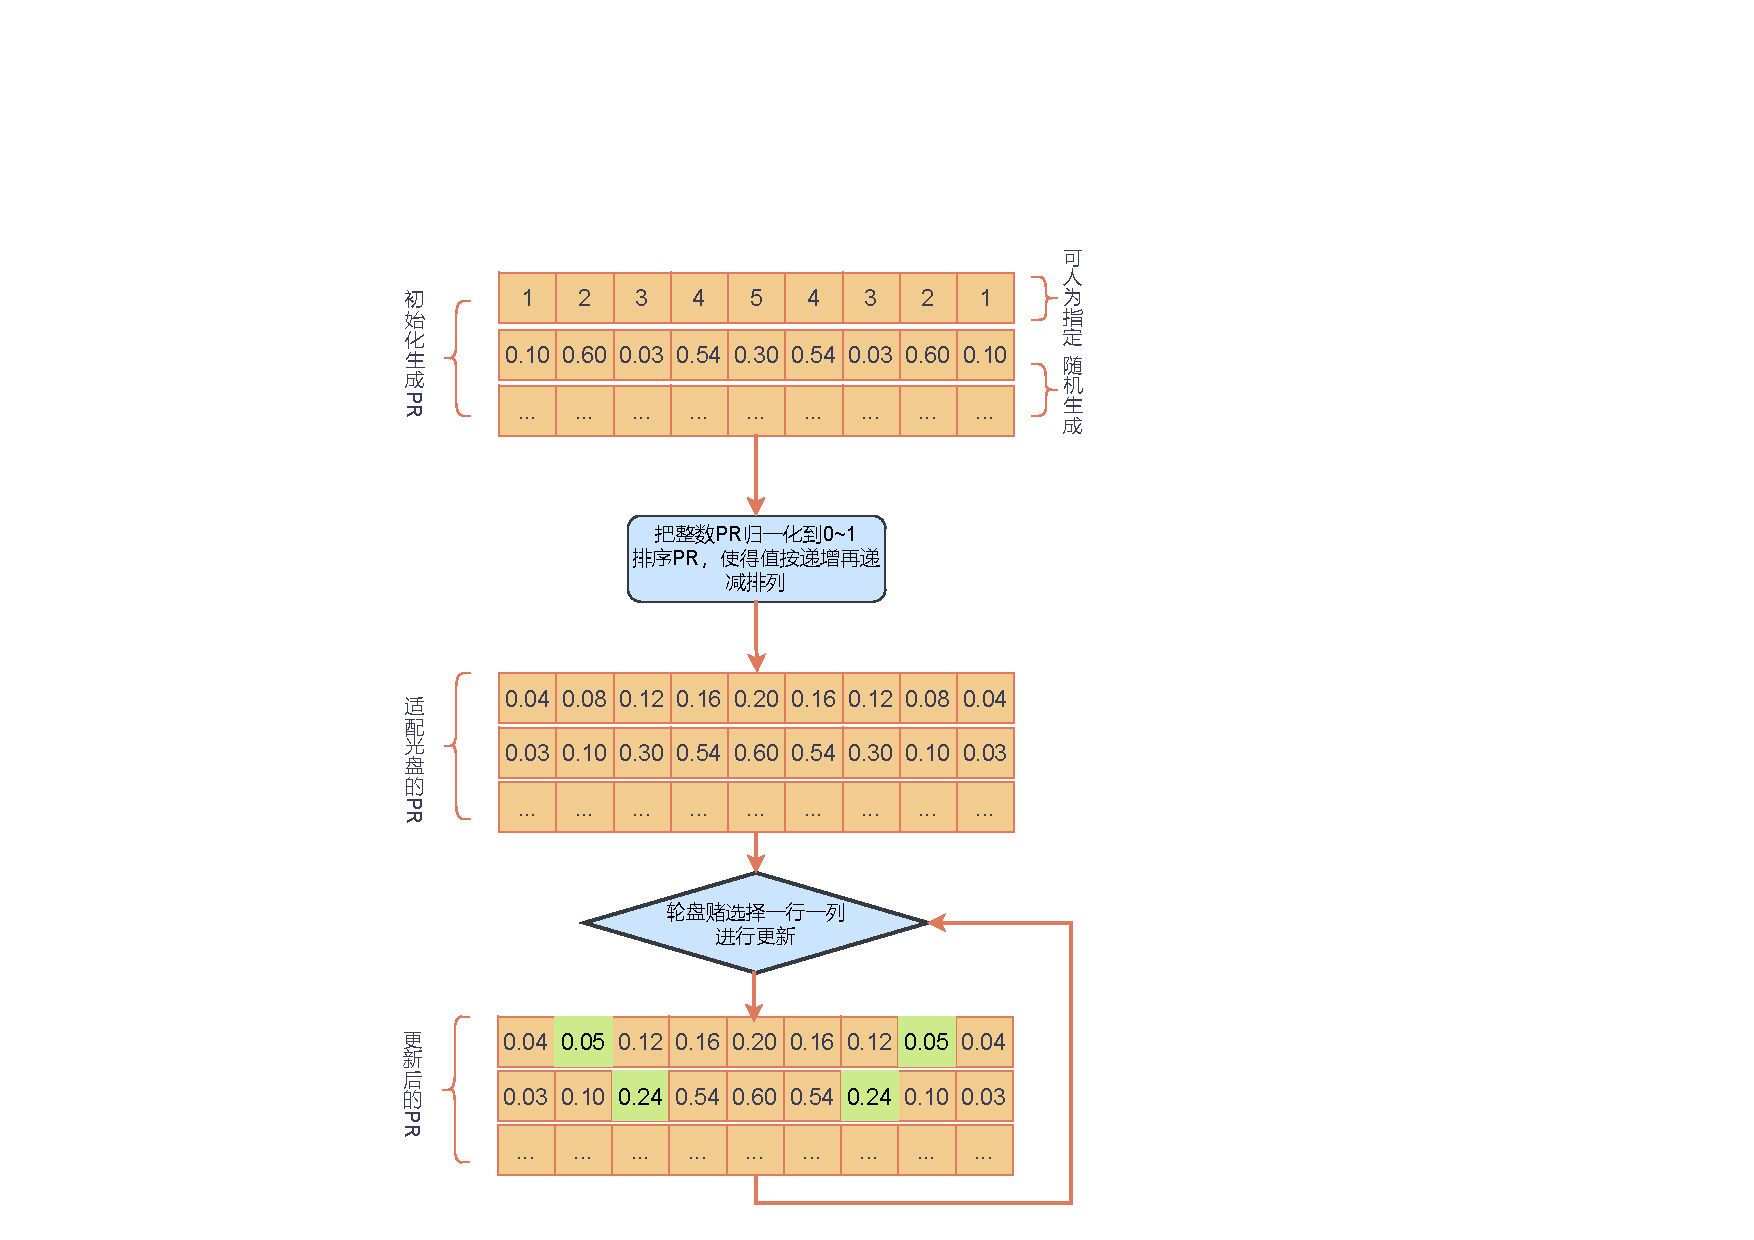
\includegraphics[width=.6\textwidth]{float/ch.cnn3/ABCPR.pdf}
	\caption{目标函数约束下PR目标的更新过程图}
	\label{fig:ABCPR}
\end{figure}

图\ref{fig:ABCPR}为在上述定制化设计下，PR目标（解）的更新过程图。雇佣蜂阶段中，每个雇佣蜂在其当前负责的PR目标邻域内进行局部搜索，生成新的候选目标，并施加约束函数以确保新解的结构合理性，随后计算新解对应的KL散度及其适应度，通过贪心策略决定是否替换原解。观察蜂阶段则基于适应度计算每个解被选择的概率，以轮盘赌方式引导更多搜索资源倾向于优质解区域，同样在邻域搜索后施加结构约束并更新解。侦察蜂阶段负责监控各解的更新状态，当某个PR目标在预设的限制次数内始终未能得到改进时，判定其陷入局部最优，随即随机生成新的候选解替代之，从而为算法注入探索活力，避免早熟收敛。通过上述各阶段的协同迭代，算法能够在全局搜索与局部开发之间取得动态平衡，最终输出一组与当前信道特性最为适配的最优PR目标。


\section{融合PR目标优化的自适应均衡系统实现}

本小节阐述引入PR目标优化后，整个均衡系统的工作流程。系统采用离线优化与在线应用相结合的运行模式：在离线优化阶段，采集代表性回读信号样本，以均衡后信号与理想信号分布的KL散度为优化目标，驱动ABC算法搜索最优PR目标；在在线应用阶段，将搜索得到的最优PR目标固化于系统中，用于指导均衡器的自适应调整与维特比检测器的判决。系统还可设计周期性优化机制，在检测到信道特性发生显著变化时触发新一轮的PR目标搜索，实现系统对长期漂移的适应能力。
s
\section{实验结果与分析}

\section{本章小结}